\documentclass[slidestop,compress,red,mathserif]{beamer}
\usepackage{ctex} %注意这个宏包
\usepackage{graphicx}
%\usepackage[bars]{beamerthemetree} % Beamer theme v 2.2
\usetheme{Warsaw} % Beamer theme v 3.0
\usecolortheme{lily} % Beamer color theme

\title{Quantifying Movie Magic with Google Search}
\author{mazefeng01@baidu.com}
\institute{Baidu, Inc}
\date{\today}

\begin{document}

\begin{frame}
\titlepage
\end{frame}

\begin{frame}
\frametitle{目录}
\tableofcontents
\end{frame}

\section{Introduction}
%%%%%%%%%%%%%%%%%%%%%%%%%%
\begin{frame}
\frametitle{Introduction}
\begin{itemize}
\pause \item This paper discuss how \textcolor{red}{search query patterns} and \textcolor{red}{paid clicks} can help us to \textcolor{red}{predict box office performance}.
\pause \item Searches in the movie category on Google are \textcolor{red}{up 56\% from 2011 to 2012.}
\pause \item Search provides a unique opportunity for film marketers to extend engagement with potential moviegoers.
\pause \item \textcolor{red}{Query volume} and \textcolor{red}{paid click volume} along with \textcolor{red}{other movie-related variables}, can predict:
	\begin{itemize}
	\pause \item A film`s opening weekend performance with \textcolor{red}{92\%} accuracy.
	\pause \item Subsequent weekend performance with \textcolor{red}{90\%} accuracy.
	\end{itemize}
\end{itemize}
\end{frame}
%%%%%%%%%%%%%%%%%%%%%%%%%%
\begin{frame}
\frametitle{Introduction}
\begin{itemize}
\pause \item \textcolor{red}{Trailer(预告片)-related search} trends \textcolor{red}{4 weeks out} from a movie release provide strong predictive power 
	for opening weekend box office revenue.
	\begin{itemize}
	\pause \item \textcolor{red}{Trailer search volume on Google} coupled with both \textcolor{red}{the franchise status of the movie(经销权) and seasonality} 
	can predict opening weekend box office revenue with \textcolor{red}{94\%} accuracy.
	\end{itemize}
\pause \item \textcolor{red}{48\%} of moviegoers decide what film to watch the day they purchase their ticket.
\end{itemize}
\end{frame}
%%%%%%%%%%%%%%%%%%%%%%%%%%
\section{The Link Between Google Search and Box Office}
%%%%%%%%%%%%%%%%%%%%%%%%%%
\begin{frame}
\frametitle{The Link Between Google Search and Box Office}
If search is a reflection of interest and intent, one would expect that the more \textcolor{red}{movie-related search activity in a given weekend, 
the bigger the box office.}
\begin{center}
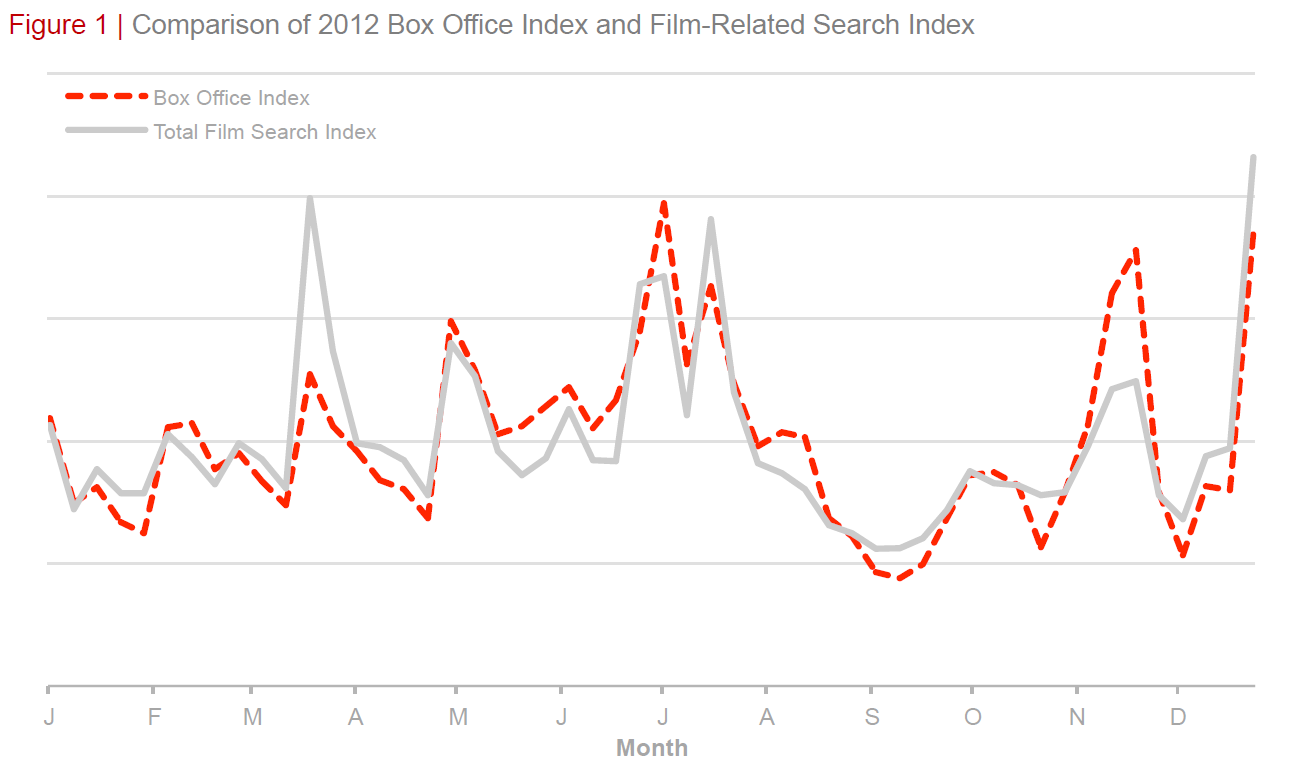
\includegraphics[height=5cm]{fig1.png}
\end{center}
\end{frame}
%%%%%%%%%%%%%%%%%%%%%%%%%%
\begin{frame}
\frametitle{The Link Between Google Search and Box Office}
If we split the overall search index into \textcolor{red}{film-specific title keywords} and \textcolor{red}{generic movie-related keywords}:
\begin{itemize}  \footnotesize
	\pause \item \textcolor{red}{Film-specific title keywords} include "[movie title]", "[movie title] trailer", "[movie title] clips", "[movie title] cast", "[movie title] tickets", "[movie title] plot", "[movie title] reviews", and other common variants related to these categories.
	\pause \item \textcolor{red}{Generic movie-related keywords} include general movie terms (e.g. "new movies", "movie showtimes"), theater chain terms (e.g., "regal showtimes", "carmike theaters"), and online movie ticket services (e.g., "fandango", "movietickets").
\end{itemize}
\end{frame}

%%%%%%%%%%%%%%%%%%%%%%%%%%
%%%%%%%%%%%%%%%%%%%%%%%%%%
\begin{frame}
\frametitle{The Link Between Google Search and Box Office}
\begin{center}
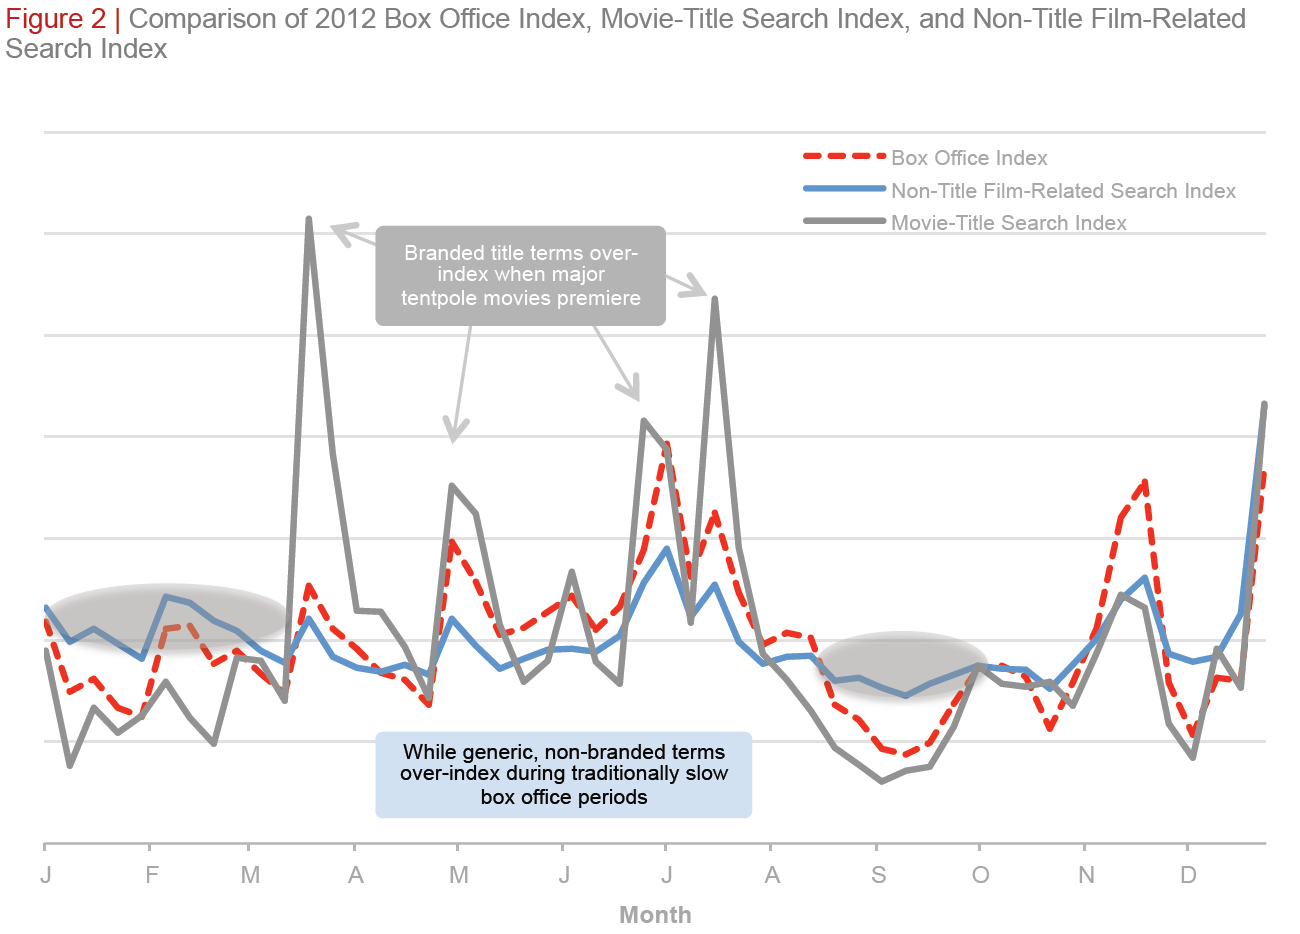
\includegraphics[width=9cm]{fig2.png}
\end{center}
\end{frame}
%%%%%%%%%%%%%%%%%%%%%%%%%%
\section{Predicting Weekend Box Office One Day Before}
%%%%%%%%%%%%%%%%%%%%%%%%%%
%%%%%%%%%%%%%%%%%%%%%%%%%%
\begin{frame}
\frametitle{Predicting Weekend Box Office One Day Before: Paid Clicks Predict Tix}
\begin{itemize}
	\pause \item 99 films released in 2012 shows that \textcolor{red}{a film`s Google search volume during the 7 days prior to its opening} is a strong indicator. 
	\pause \item A simple linear regression model using film-related search query volume as a predictor of weekend box office performance yields an \textcolor{red}{$R^2$=70\%.}
	\pause \item In other words,  \textcolor{red}{70\% of the variation in box office performance can be explained with search query volume.}
\end{itemize}
\end{frame}
%%%%%%%%%%%%%%%%%%%%%%%%%%
%%%%%%%%%%%%%%%%%%%%%%%%%%
\begin{frame}
\frametitle{Predicting Weekend Box Office One Day Before: Paid Clicks Predict Tix}
\begin{center}
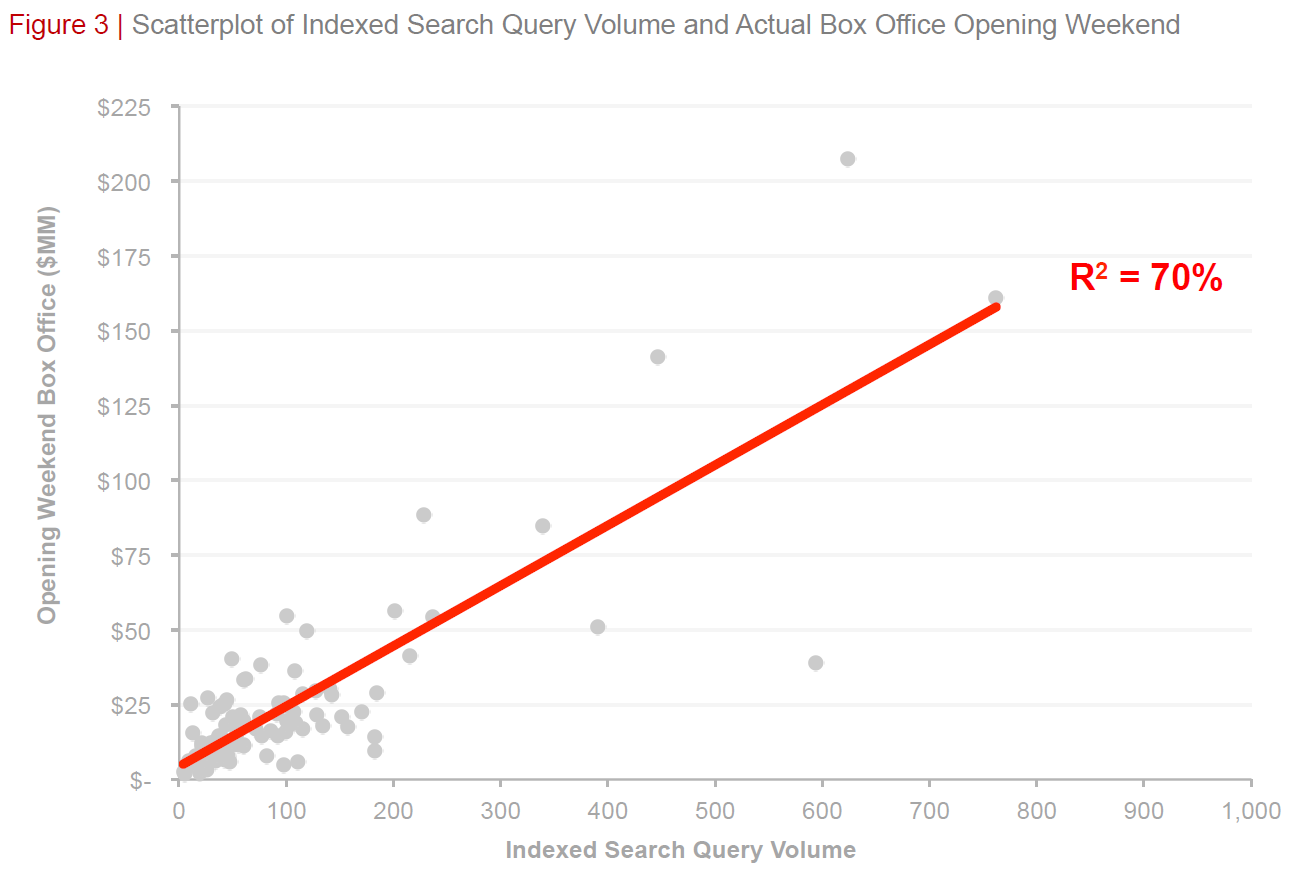
\includegraphics[width=9cm]{fig3.png}
\end{center}
\end{frame}
%%%%%%%%%%%%%%%%%%%%%%%%%%
%%%%%%%%%%%%%%%%%%%%%%%%%%
\begin{frame}
\frametitle{Predicting Weekend Box Office One Day Before: Paid Clicks Predict Tix}
\begin{itemize}
	\pause \item  \textcolor{red}{Search ad click volume} is a key element of the prediction model as it signifies deeper engagement with a particular film.
	\pause \item After examing over 30 different film variables, non-statistically significant variables were dropped, resulting in a model that includes the following variables:
	\begin{enumerate}
		\pause \item \textcolor{red}{Search query volume (seven-day period prior to release date)}
		\pause \item \textcolor{red}{Search ad click volume (seven-day period prior to release date)}
		\pause \item \textcolor{red}{Theater count}
		\pause \item \textcolor{red}{Franchise(经销权) status}
	\end{enumerate}
\end{itemize}
\end{frame}
%%%%%%%%%%%%%%%%%%%%%%%%%%
%%%%%%%%%%%%%%%%%%%%%%%%%%
\begin{frame}
\frametitle{Predicting Weekend Box Office One Day Before: Paid Clicks Predict Tix}
\begin{center}
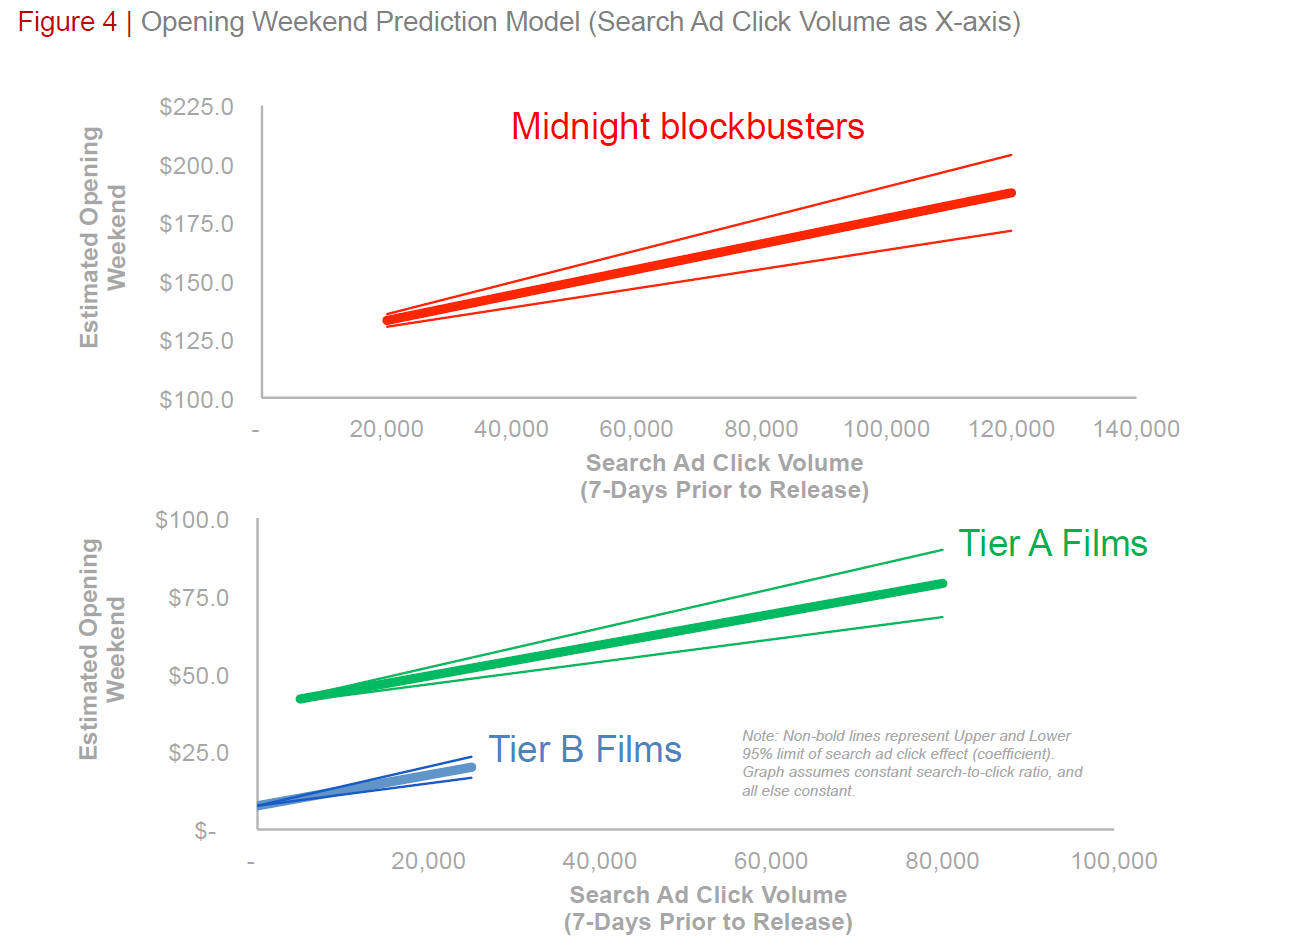
\includegraphics[width=9cm]{fig4.png}
\end{center}
\end{frame}
%%%%%%%%%%%%%%%%%%%%%%%%%%
%%%%%%%%%%%%%%%%%%%%%%%%%%
\begin{frame}
\frametitle{Predicting Weekend Box Office One Day Before: Paid Clicks Predict Tix}
\begin{itemize}
	\pause \item This model has an $R^2$ of \textcolor{red}{92\%}, meaning box office sales can be predicted by the combination of the aforementioned variables with 92\% accuracy.
	\pause \item In the \textcolor{red}{7 day window prior} to a film`s release date: 
	\begin{enumerate}
		\pause \item If one film has \textcolor{red}{250,000 more search queries} than a similar film, 
			the film with more queries is likely to perform up to \textcolor{red}{\$4.3M} better.
		\pause \item If a film has \textcolor{red}{20,000 more paid clicks} than a similar film, 
			it is expected to bring in up to \textcolor{red}{\$7.5M} more.
	\end{enumerate}
\end{itemize}
\end{frame}
%%%%%%%%%%%%%%%%%%%%%%%%%%
%%%%%%%%%%%%%%%%%%%%%%%%%%
\begin{frame}
\frametitle{Predicting Weekend Box Office One Day Before: Paid Clicks Predict Tix}
\begin{itemize}
	\pause \item \textcolor{red}{Beyond Opening Weekend}: \textcolor{red}{the number of paid clicks a film garners} along with other film-related metrics, 
	serve as strong indicators of how a film will fare in a post-opening weekend.
	\pause \item For holdover films (i.e. films in their second week or beyond), the significant variables in our regression model include:
	\begin{enumerate}
		\pause \item \textcolor{red}{Search ad clicks (Monday-Thursday prior to weekend)}
		\pause \item \textcolor{red}{Theater count}
		\pause \item \textcolor{red}{Previous weekend performance}
		\pause \item \textcolor{red}{Rotten Tomatoes audience score}
	\end{enumerate}
\end{itemize}
\end{frame}
%%%%%%%%%%%%%%%%%%%%%%%%%%
%%%%%%%%%%%%%%%%%%%%%%%%%%
\begin{frame}
\frametitle{Predicting Weekend Box Office One Day Before: Paid Clicks Predict Tix}
\begin{center}
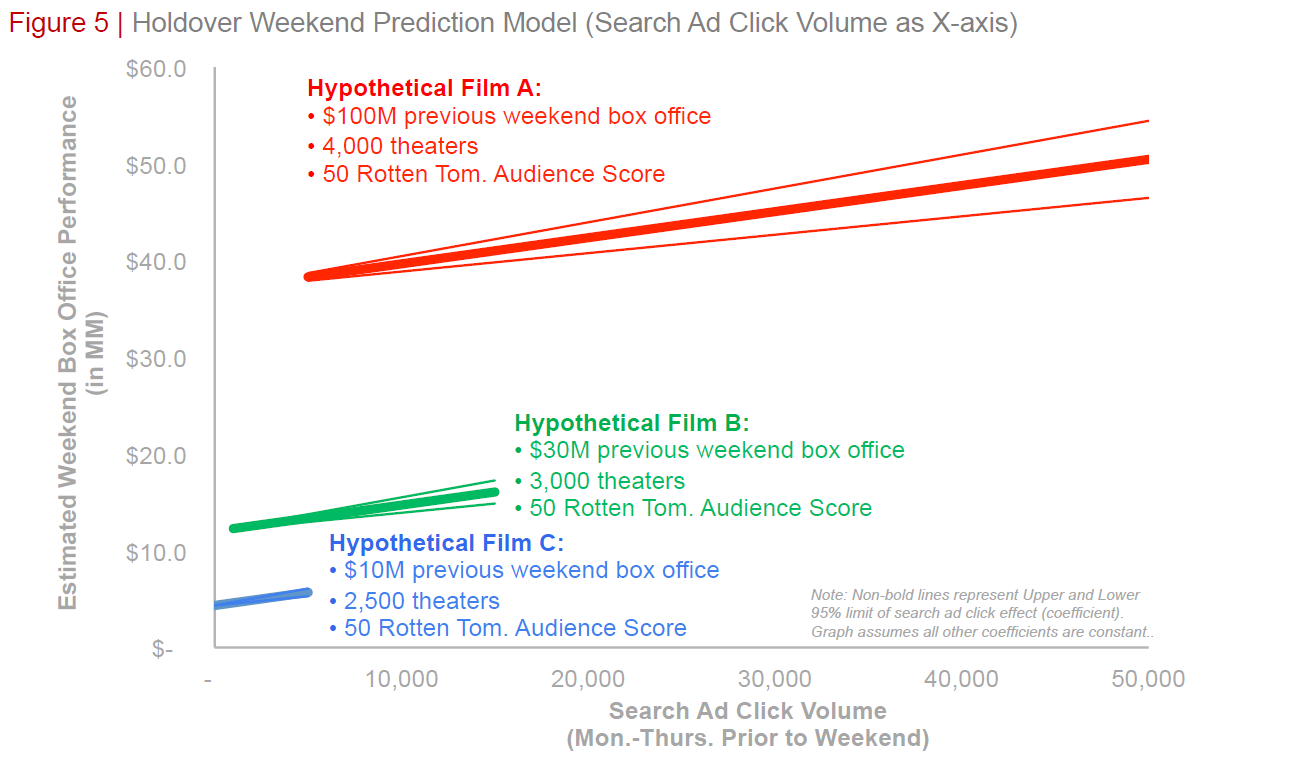
\includegraphics[width=9cm]{fig5.png}
\end{center}
\end{frame}
%%%%%%%%%%%%%%%%%%%%%%%%%%
%%%%%%%%%%%%%%%%%%%%%%%%%%
\begin{frame}
\frametitle{Predicting Weekend Box Office One Day Before: Paid Clicks Predict Tix}
\begin{itemize}
	\pause \item \textcolor{red}{Search query volume for holdover films} is \textcolor{red}{not} a significant factor in predicting box office performance after opening weekend, while \textcolor{red}{search ad clicks} remain a strong indicator.
	\begin{itemize}
		\pause \item Once a film has opened, search ad clicks are a strong sign of intent to purchase a ticket.
		\pause \item The intent associated with a search query is more varied.
	\end{itemize}
	\pause \item If one film garners \textcolor{red}{10,000 more paid clicks}  is likely to perform approximately \textcolor{red}{$1.9-$3.5M} better.
\end{itemize}
\end{frame}
%%%%%%%%%%%%%%%%%%%%%%%%%%
%%%%%%%%%%%%%%%%%%%%%%%%%%
\section{Predicting Box Office One-Month Before Release}
%%%%%%%%%%%%%%%%%%%%%%%%%%
%%%%%%%%%%%%%%%%%%%%%%%%%%
\begin{frame}
\frametitle{Predicting Box Office One-Month Before Release: In Trailer Searches We Trust}
\begin{itemize}
	\pause \item Leave movie marketers with very much time to react and adjust their marketing campaigns in the pre-release time frame.
	\pause \item  \textcolor{red}{Overall title search volume loses some of its predictive power} the further it is from premiere date.
	\pause \item The key to long-range box office forecasting lies in movie trailer engagement,  \textcolor{red}{trailer-related search query volume} holds strong predictive power.
\end{itemize}
\end{frame}
%%%%%%%%%%%%%%%%%%%%%%%%%%
%%%%%%%%%%%%%%%%%%%%%%%%%%
\begin{frame}
\frametitle{Predicting Box Office One-Month Before Release: In Trailer Searches We Trust}
\begin{itemize}
	\pause \item \textcolor{red}{The number of trailer searches} mattered most in terms of predicting box office four weeks prior to a film`s release week (\textcolor{red}{$R^2$ = 62\%}).
	\pause \item Similar to trailer-related Google searches,  \textcolor{red}{title-related searches on YouTube} have the highest predictive power four weeks from release date (\textcolor{red}{$R^2$ = 55\%}).
	\pause \item \textcolor{red}{94\%} of variation in a film`s box office opening can be explained with trailer-related title search volume 4 weeks prior to release, coupled with seasonality and franchise status.
\end{itemize}
\end{frame}
%%%%%%%%%%%%%%%%%%%%%%%%%%
% [allowframebreaks]
%%%%%%%%%%%%%%%%%%%%%%%%%%
\begin{frame}
\frametitle{Predicting Box Office One-Month Before Release: In Trailer Searches We Trust}
\begin{center}
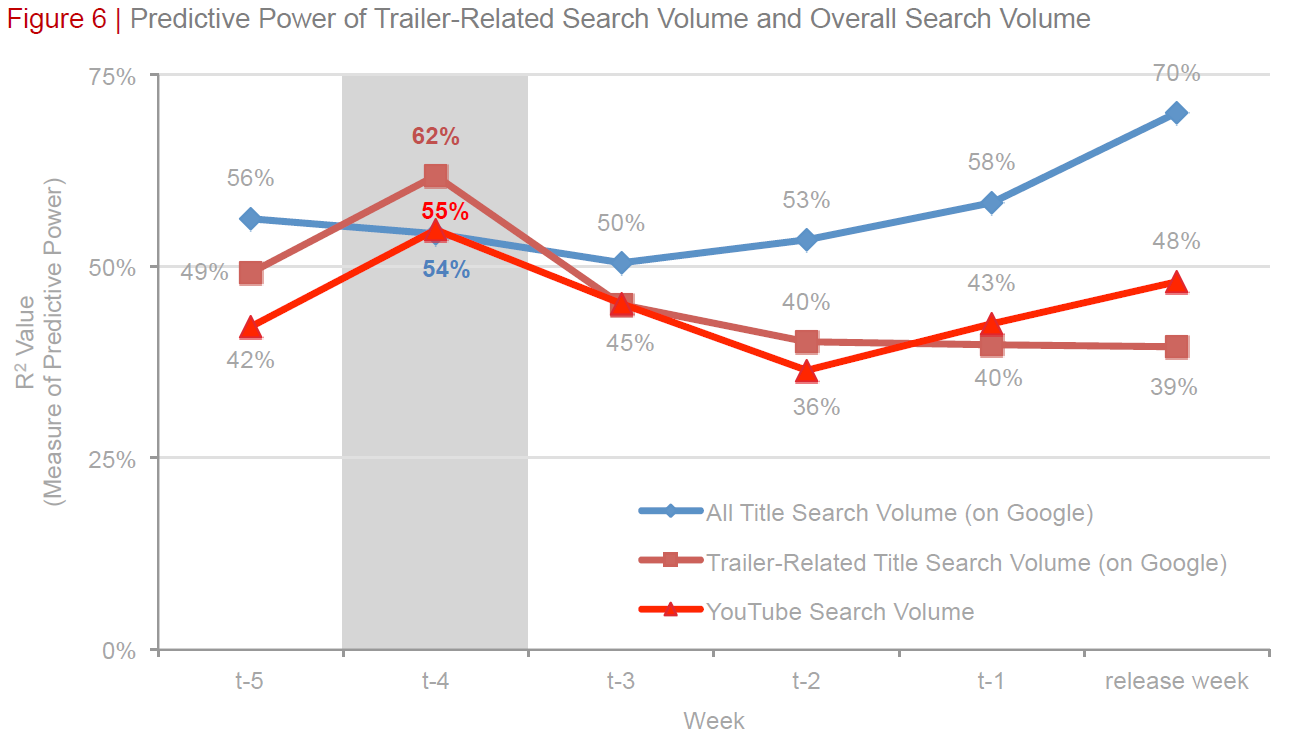
\includegraphics[width=9cm]{fig6.png}
\end{center}
\end{frame}
%%%%%%%%%%%%%%%%%%%%%%%%%%
%%%%%%%%%%%%%%%%%%%%%%%%%%

\end{document}